\documentclass[11pt, oneside]{article}   	% use "amsart" instead of "article" for AMSLaTeX format
\usepackage{geometry}                		% See geometry.pdf to learn the layout options. There are lots.
\geometry{letterpaper}                   		% ... or a4paper or a5paper or ... 
%\geometry{landscape}                		% Activate for for rotated page geometry
%\usepackage[parfill]{parskip}    		% Activate to begin paragraphs with an empty line rather than an indent
\usepackage{graphicx}				% Use pdf, png, jpg, or eps§ with pdflatex; use eps in DVI mode
\usepackage{tikz}								% TeX will automatically convert eps --> pdf in pdflatex
\usetikzlibrary{arrows}		
\usepackage{amssymb}

\title{Brief Article}
\author{The Author}
%\date{}							% Activate to display a given date or no date

\begin{document}
\maketitle
%\section{}
%\subsection{}

\section{question 2}

%%%%%%%%%%%%%%%%%%%%%%%%%%%%%%%%%%%%%%%%%%

\clearpage

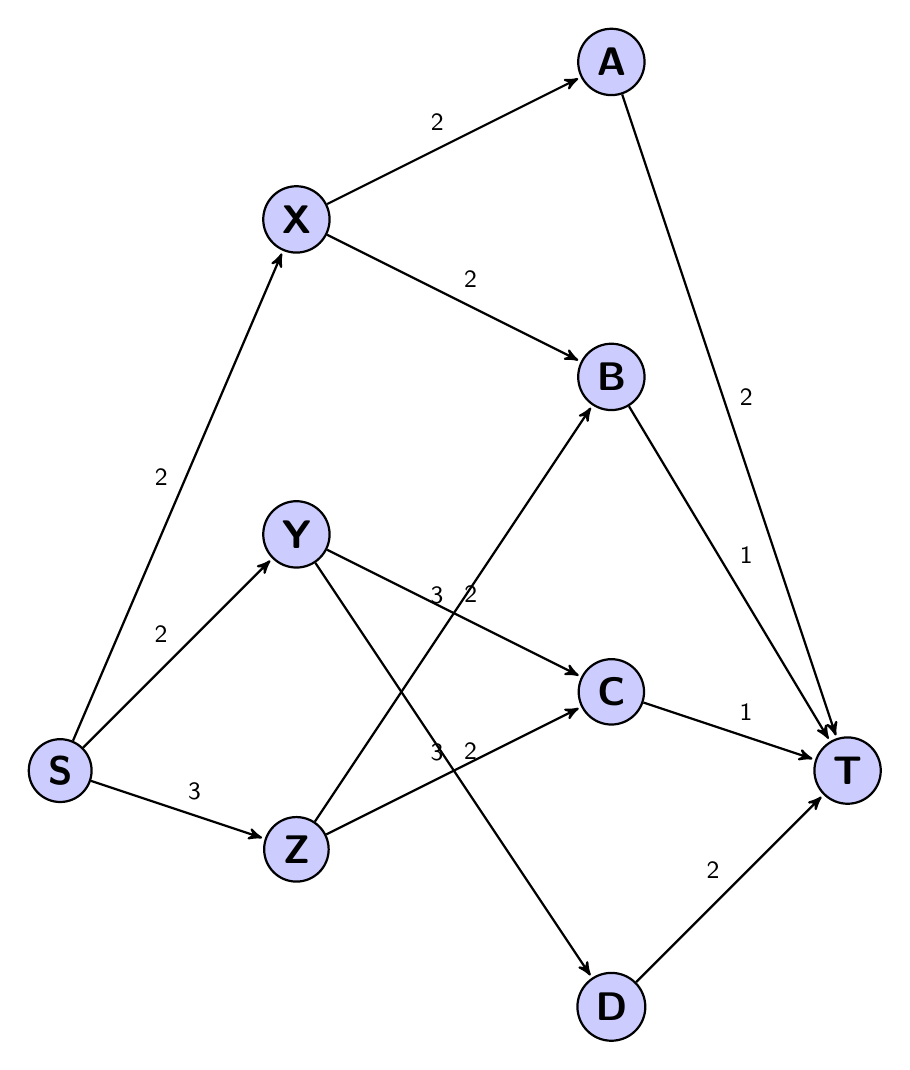
\begin{tikzpicture}[->,>=stealth',shorten >=1pt,auto,node distance=3cm,thick,main node/.style={circle,fill=blue!20,draw,font=\sffamily\Large\bfseries}]
  \node[main node] (1) at (5,5) {S};
  \node[main node] (2) at (8,12) {X};
  \node[main node] (3) at (8,8) {Y};
  \node[main node] (4) at (8,4) {Z};
  \node[main node] (5) at (12,14) {A};
  \node[main node] (6) at (12,10) {B};
  \node[main node] (7) at (12,6) {C};
  \node[main node] (8) at (12,2) {D};
  \node[main node] (9) at (15,5) {T};

\path[every node/.style={font=\sffamily\small}]
  (1) edge node {2} (2)
  (1) edge node {2} (3)
  (1) edge node {3} (4)
  (2) edge node {2} (5)
  (2) edge node {2} (6)
  (3) edge node {2} (7)
  (3) edge node {2} (8)
  (4) edge node {3} (6)
  (4) edge node {3} (7)
  (5) edge node {2} (9)
  (6) edge node {1} (9)
  (7) edge node {1} (9)
  (8) edge node {2} (9)
;
\end{tikzpicture}


\clearpage

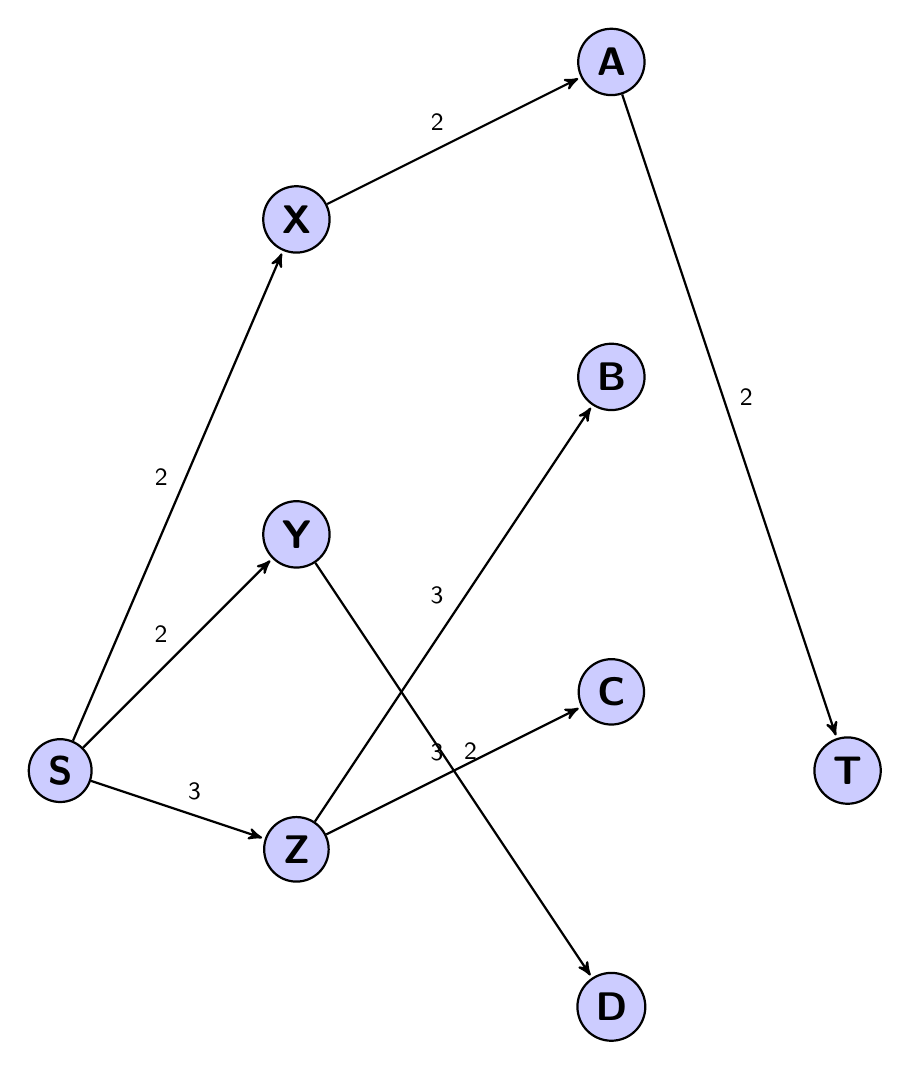
\begin{tikzpicture}[->,>=stealth',shorten >=1pt,auto,node distance=3cm,thick,main node/.style={circle,fill=blue!20,draw,font=\sffamily\Large\bfseries}]
  \node[main node] (1) at (5,5) {S};
  \node[main node] (2) at (8,12) {X};
  \node[main node] (3) at (8,8) {Y};
  \node[main node] (4) at (8,4) {Z};
  \node[main node] (5) at (12,14) {A};
  \node[main node] (6) at (12,10) {B};
  \node[main node] (7) at (12,6) {C};
  \node[main node] (8) at (12,2) {D};
  \node[main node] (9) at (15,5) {T};

\path[every node/.style={font=\sffamily\small}]
  (1) edge node {2} (2)
  (1) edge node {2} (3)
  (1) edge node {3} (4)
  (2) edge node {2} (5)
  (4) edge node {3} (6)
  (4) edge node {3} (7)
  (3) edge node {2} (8)
  (5) edge node {2} (9)
;
\end{tikzpicture}

\clearpage
path:1 2 5 9 
\\
capacity:2

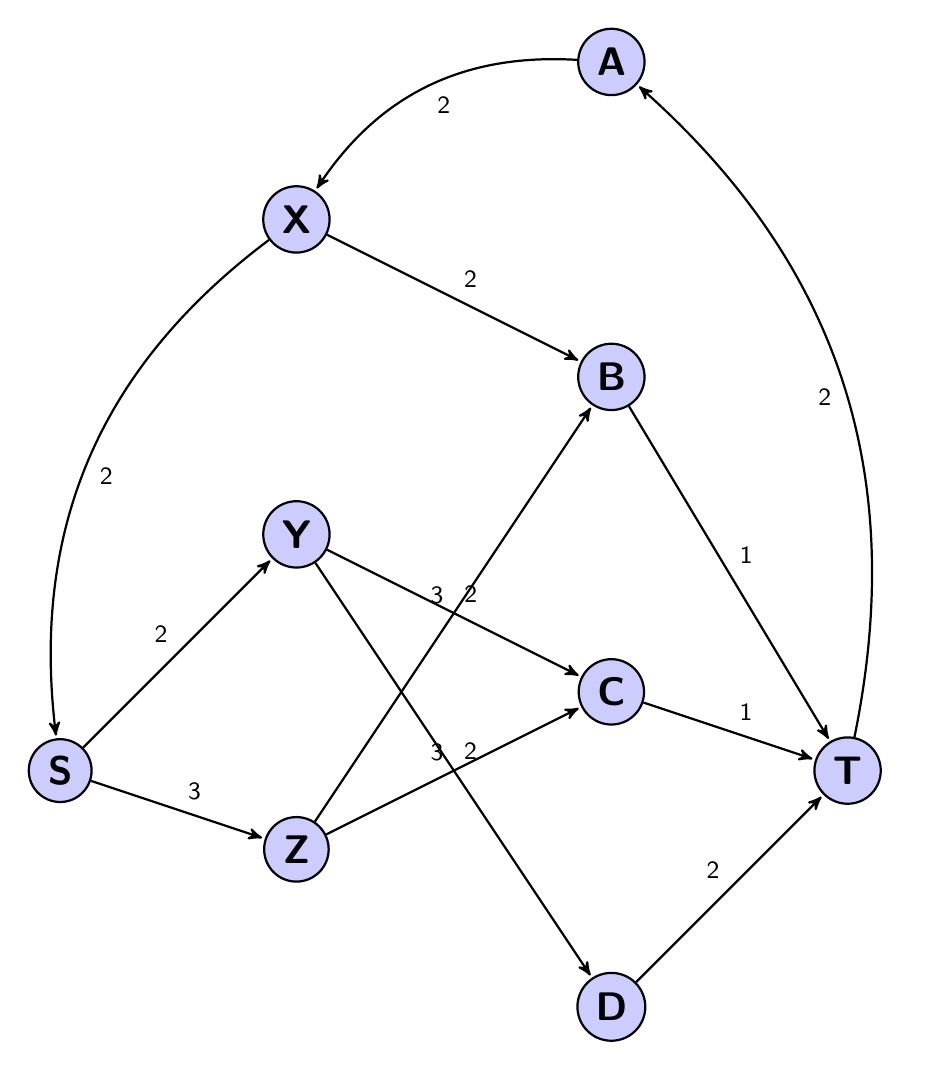
\begin{tikzpicture}[->,>=stealth',shorten >=1pt,auto,node distance=3cm,thick,main node/.style={circle,fill=blue!20,draw,font=\sffamily\Large\bfseries}]
  \node[main node] (1) at (5,5) {S};
  \node[main node] (2) at (8,12) {X};
  \node[main node] (3) at (8,8) {Y};
  \node[main node] (4) at (8,4) {Z};
  \node[main node] (5) at (12,14) {A};
  \node[main node] (6) at (12,10) {B};
  \node[main node] (7) at (12,6) {C};
  \node[main node] (8) at (12,2) {D};
  \node[main node] (9) at (15,5) {T};

\path[every node/.style={font=\sffamily\small}]
  (1) edge node {2} (3)
  (1) edge node {3} (4)
  (2) edge node {2} (6)
  (3) edge node {2} (7)
  (3) edge node {2} (8)
  (4) edge node {3} (6)
  (4) edge node {3} (7)
  (6) edge node {1} (9)
  (7) edge node {1} (9)
  (8) edge node {2} (9)
  (9) edge [bend right] node  {2} (5)
  (2) edge [bend right] node  {2} (1)
  (5) edge [bend right] node  {2} (2)
;
\end{tikzpicture}


\clearpage

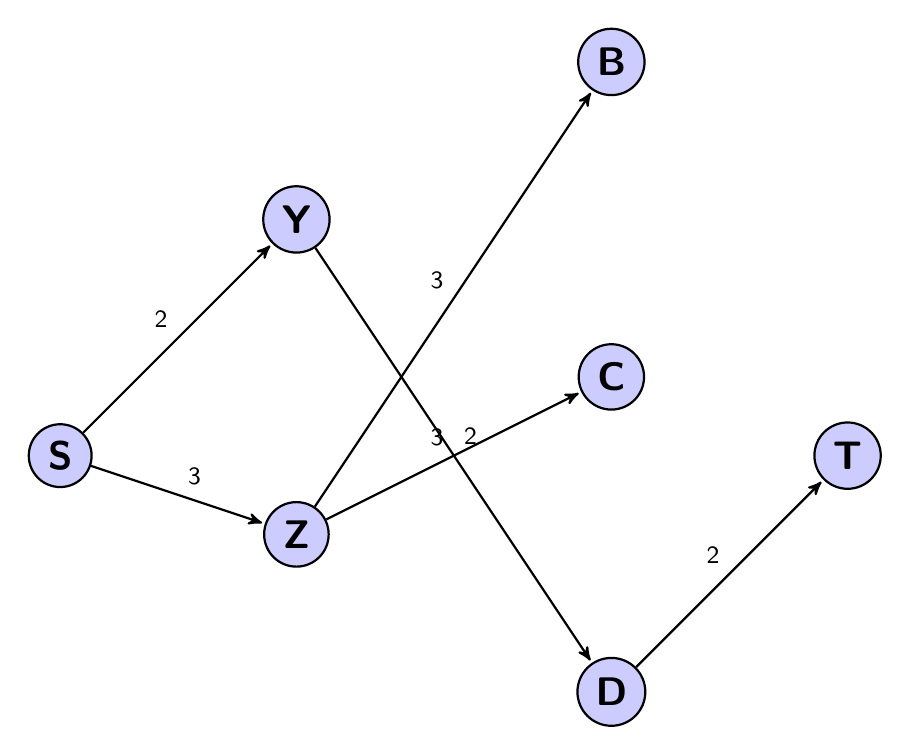
\begin{tikzpicture}[->,>=stealth',shorten >=1pt,auto,node distance=3cm,thick,main node/.style={circle,fill=blue!20,draw,font=\sffamily\Large\bfseries}]
  \node[main node] (1) at (5,5) {S};
  \node[main node] (3) at (8,8) {Y};
  \node[main node] (4) at (8,4) {Z};
  \node[main node] (6) at (12,10) {B};
  \node[main node] (7) at (12,6) {C};
  \node[main node] (8) at (12,2) {D};
  \node[main node] (9) at (15,5) {T};

\path[every node/.style={font=\sffamily\small}]
  (1) edge node {2} (3)
  (1) edge node {3} (4)
  (4) edge node {3} (6)
  (4) edge node {3} (7)
  (3) edge node {2} (8)
  (8) edge node {2} (9)
;
\end{tikzpicture}

\clearpage
path:1 3 8 9 
\\
capacity:2

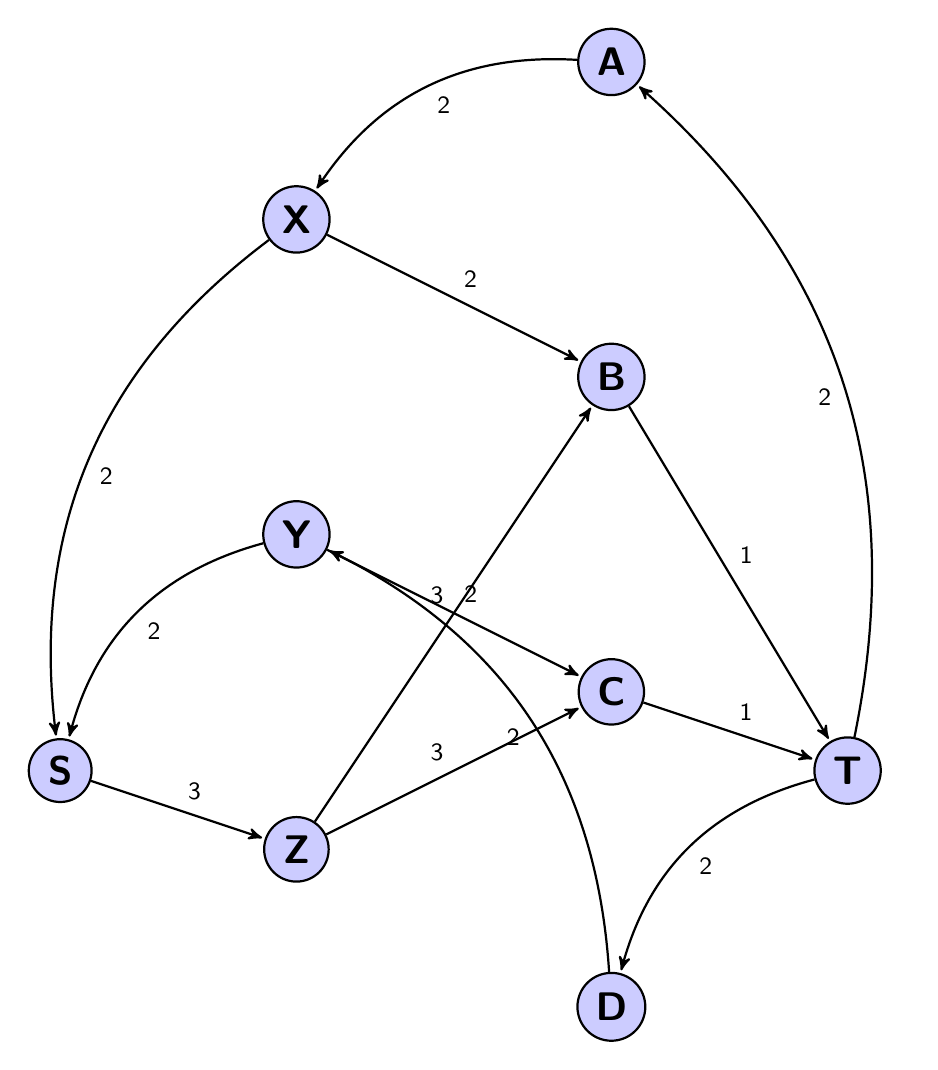
\begin{tikzpicture}[->,>=stealth',shorten >=1pt,auto,node distance=3cm,thick,main node/.style={circle,fill=blue!20,draw,font=\sffamily\Large\bfseries}]
  \node[main node] (1) at (5,5) {S};
  \node[main node] (2) at (8,12) {X};
  \node[main node] (3) at (8,8) {Y};
  \node[main node] (4) at (8,4) {Z};
  \node[main node] (5) at (12,14) {A};
  \node[main node] (6) at (12,10) {B};
  \node[main node] (7) at (12,6) {C};
  \node[main node] (8) at (12,2) {D};
  \node[main node] (9) at (15,5) {T};

\path[every node/.style={font=\sffamily\small}]
  (1) edge node {3} (4)
  (2) edge node {2} (6)
  (3) edge node {2} (7)
  (4) edge node {3} (6)
  (4) edge node {3} (7)
  (6) edge node {1} (9)
  (7) edge node {1} (9)
  (9) edge [bend right] node  {2} (8)
  (9) edge [bend right] node  {2} (5)
  (2) edge [bend right] node  {2} (1)
  (3) edge [bend right] node  {2} (1)
  (5) edge [bend right] node  {2} (2)
  (8) edge [bend right] node  {2} (3)
;
\end{tikzpicture}


\clearpage

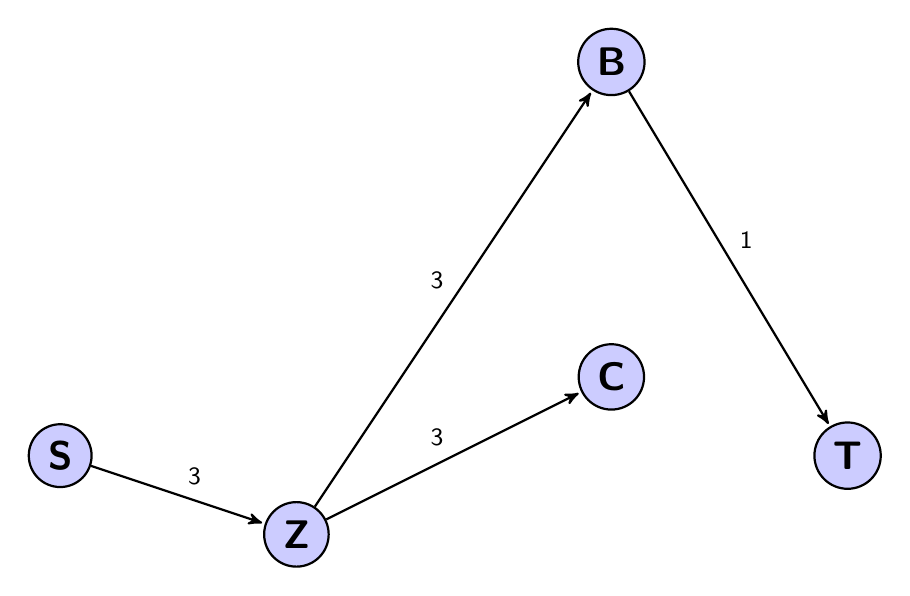
\begin{tikzpicture}[->,>=stealth',shorten >=1pt,auto,node distance=3cm,thick,main node/.style={circle,fill=blue!20,draw,font=\sffamily\Large\bfseries}]
  \node[main node] (1) at (5,5) {S};
  \node[main node] (4) at (8,4) {Z};
  \node[main node] (6) at (12,10) {B};
  \node[main node] (7) at (12,6) {C};
  \node[main node] (9) at (15,5) {T};

\path[every node/.style={font=\sffamily\small}]
  (1) edge node {3} (4)
  (4) edge node {3} (6)
  (4) edge node {3} (7)
  (6) edge node {1} (9)
;
\end{tikzpicture}

\clearpage
path:1 4 6 9 
\\
capacity:1

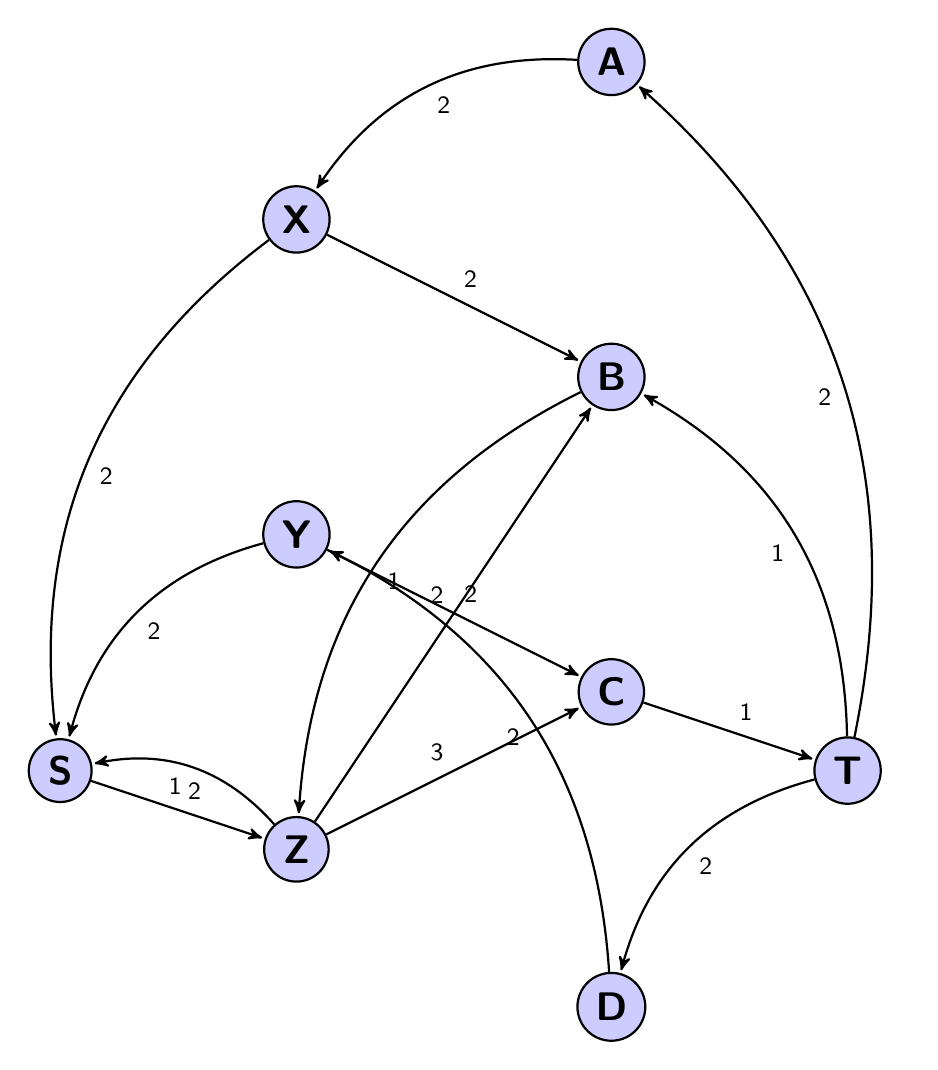
\begin{tikzpicture}[->,>=stealth',shorten >=1pt,auto,node distance=3cm,thick,main node/.style={circle,fill=blue!20,draw,font=\sffamily\Large\bfseries}]
  \node[main node] (1) at (5,5) {S};
  \node[main node] (2) at (8,12) {X};
  \node[main node] (3) at (8,8) {Y};
  \node[main node] (4) at (8,4) {Z};
  \node[main node] (5) at (12,14) {A};
  \node[main node] (6) at (12,10) {B};
  \node[main node] (7) at (12,6) {C};
  \node[main node] (8) at (12,2) {D};
  \node[main node] (9) at (15,5) {T};

\path[every node/.style={font=\sffamily\small}]
  (1) edge node {2} (4)
  (2) edge node {2} (6)
  (3) edge node {2} (7)
  (4) edge node {2} (6)
  (4) edge node {3} (7)
  (7) edge node {1} (9)
  (4) edge [bend right] node  {1} (1)
  (9) edge [bend right] node  {2} (8)
  (9) edge [bend right] node  {2} (5)
  (2) edge [bend right] node  {2} (1)
  (3) edge [bend right] node  {2} (1)
  (5) edge [bend right] node  {2} (2)
  (8) edge [bend right] node  {2} (3)
  (6) edge [bend right] node  {1} (4)
  (9) edge [bend right] node  {1} (6)
;
\end{tikzpicture}


\clearpage

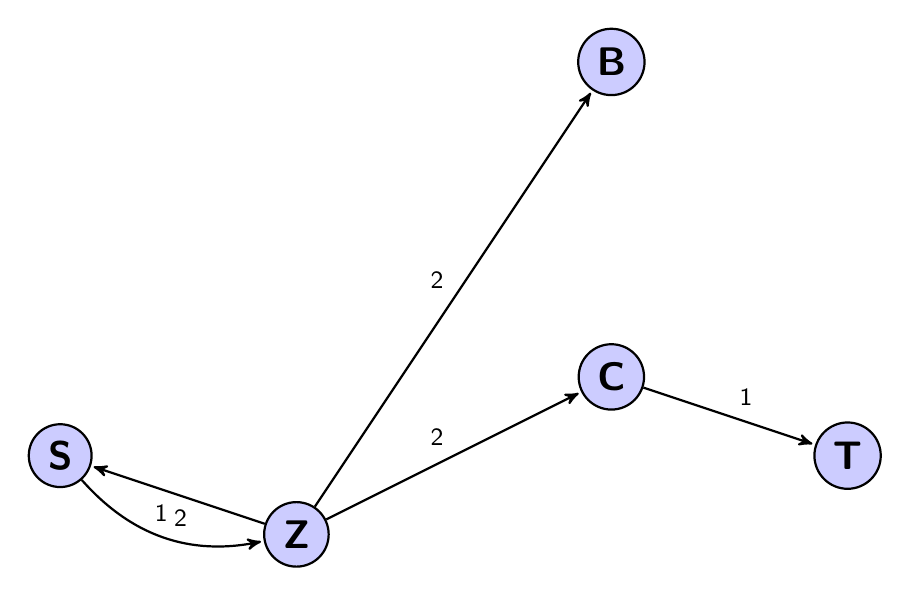
\begin{tikzpicture}[->,>=stealth',shorten >=1pt,auto,node distance=3cm,thick,main node/.style={circle,fill=blue!20,draw,font=\sffamily\Large\bfseries}]
  \node[main node] (1) at (5,5) {S};
  \node[main node] (4) at (8,4) {Z};
  \node[main node] (6) at (12,10) {B};
  \node[main node] (7) at (12,6) {C};
  \node[main node] (9) at (15,5) {T};

\path[every node/.style={font=\sffamily\small}]
  (4) edge node {1} (1)
  (1) edge [bend right] node  {2} (4)
  (4) edge node {2} (6)
  (4) edge node {2} (7)
  (7) edge node {1} (9)
;
\end{tikzpicture}

\clearpage
path:1 4 7 9 
\\
capacity:1

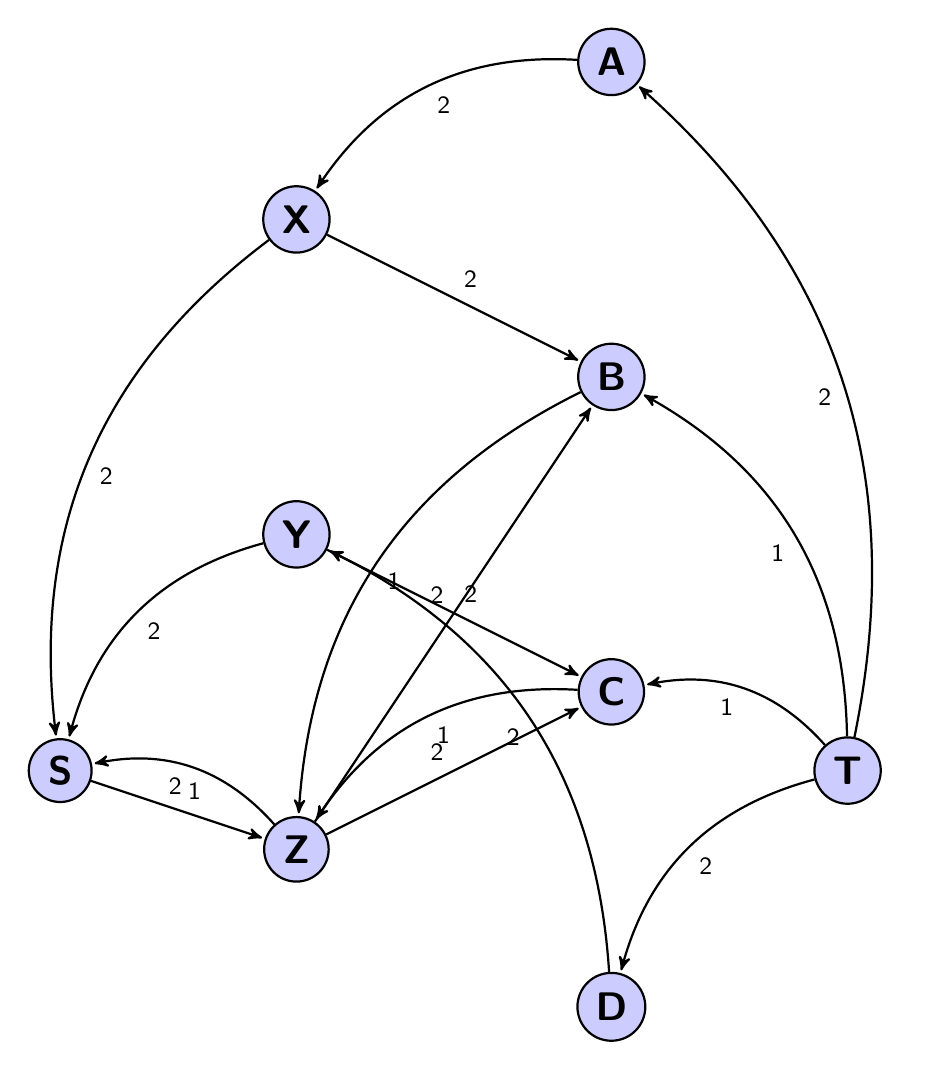
\begin{tikzpicture}[->,>=stealth',shorten >=1pt,auto,node distance=3cm,thick,main node/.style={circle,fill=blue!20,draw,font=\sffamily\Large\bfseries}]
  \node[main node] (1) at (5,5) {S};
  \node[main node] (2) at (8,12) {X};
  \node[main node] (3) at (8,8) {Y};
  \node[main node] (4) at (8,4) {Z};
  \node[main node] (5) at (12,14) {A};
  \node[main node] (6) at (12,10) {B};
  \node[main node] (7) at (12,6) {C};
  \node[main node] (8) at (12,2) {D};
  \node[main node] (9) at (15,5) {T};

\path[every node/.style={font=\sffamily\small}]
  (1) edge node {1} (4)
  (2) edge node {2} (6)
  (3) edge node {2} (7)
  (4) edge node {2} (6)
  (4) edge node {2} (7)
  (4) edge [bend right] node  {2} (1)
  (9) edge [bend right] node  {2} (8)
  (9) edge [bend right] node  {1} (7)
  (9) edge [bend right] node  {2} (5)
  (2) edge [bend right] node  {2} (1)
  (3) edge [bend right] node  {2} (1)
  (5) edge [bend right] node  {2} (2)
  (8) edge [bend right] node  {2} (3)
  (6) edge [bend right] node  {1} (4)
  (7) edge [bend right] node  {1} (4)
  (9) edge [bend right] node  {1} (6)
;
\end{tikzpicture}

6

%%%%%%%%%%%%%%%%%%%%%%%%%%%%%%%%%%%%%%%%%%

\section{question 3}

%%%%%%%%%%%%%%%%%%%%%%%%%%%%%%%%%%%%%%%%%%

\clearpage

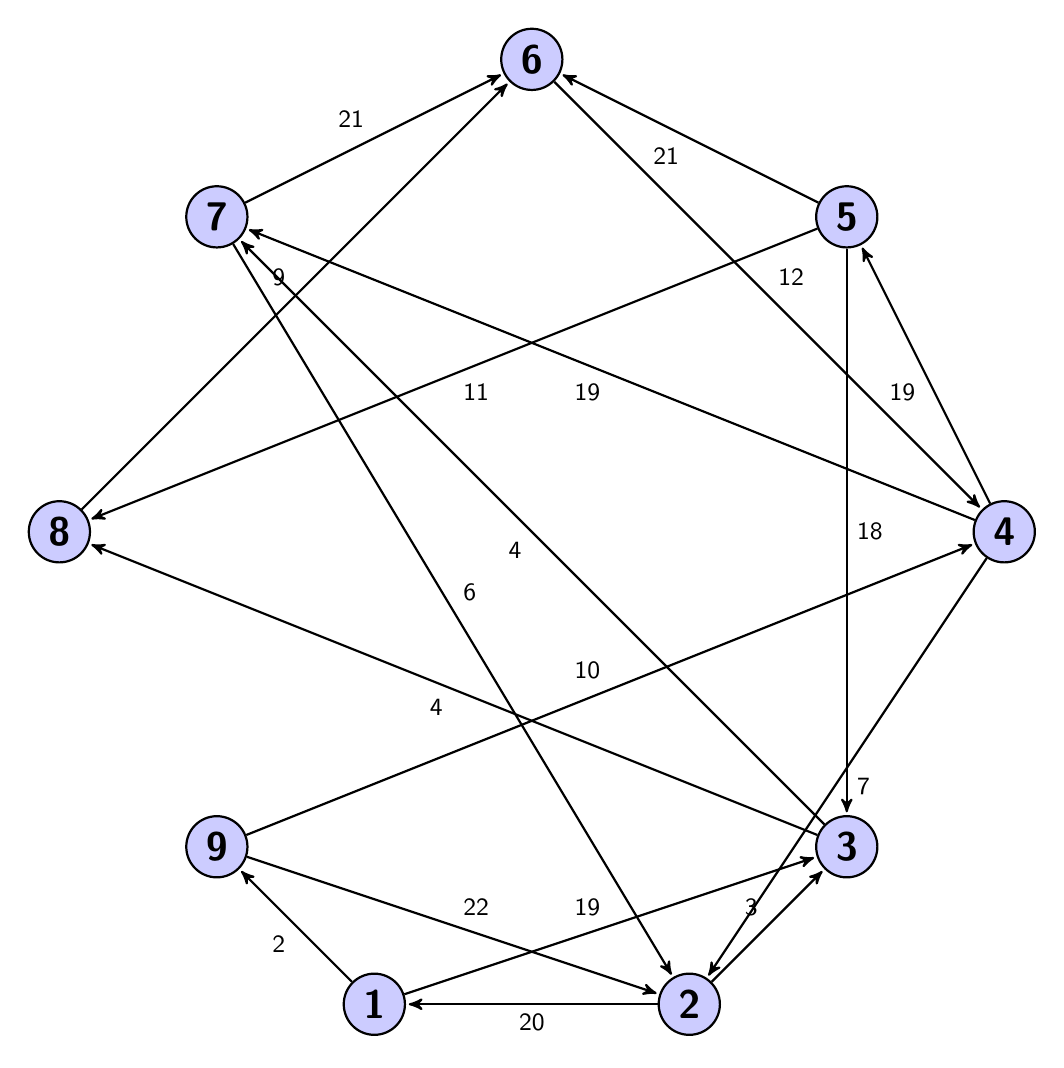
\begin{tikzpicture}[->,>=stealth',shorten >=1pt,auto,node distance=3cm,thick,main node/.style={circle,fill=blue!20,draw,font=\sffamily\Large\bfseries}]
  \node[main node] (1) at (10,0) {1};
  \node[main node] (2) at (14,0) {2};
  \node[main node] (3) at (16,2) {3};
  \node[main node] (4) at (18,6) {4};
  \node[main node] (5) at (16,10) {5};
  \node[main node] (6) at (12,12) {6};
  \node[main node] (7) at (8,10) {7};
  \node[main node] (8) at (6,6) {8};
  \node[main node] (9) at (8,2) {9};

\path[every node/.style={font=\sffamily\small}]
  (1) edge node {19} (3)
  (1) edge node {2} (9)
  (2) edge node {20} (1)
  (2) edge node {3} (3)
  (3) edge node {4} (7)
  (3) edge node {4} (8)
  (4) edge node {7} (2)
  (4) edge node {19} (5)
  (4) edge node {19} (7)
  (5) edge node {18} (3)
  (5) edge node {21} (6)
  (5) edge node {11} (8)
  (6) edge node {12} (4)
  (7) edge node {6} (2)
  (7) edge node {21} (6)
  (8) edge node {9} (6)
  (9) edge node {22} (2)
  (9) edge node {10} (4)
;
\end{tikzpicture}


\clearpage

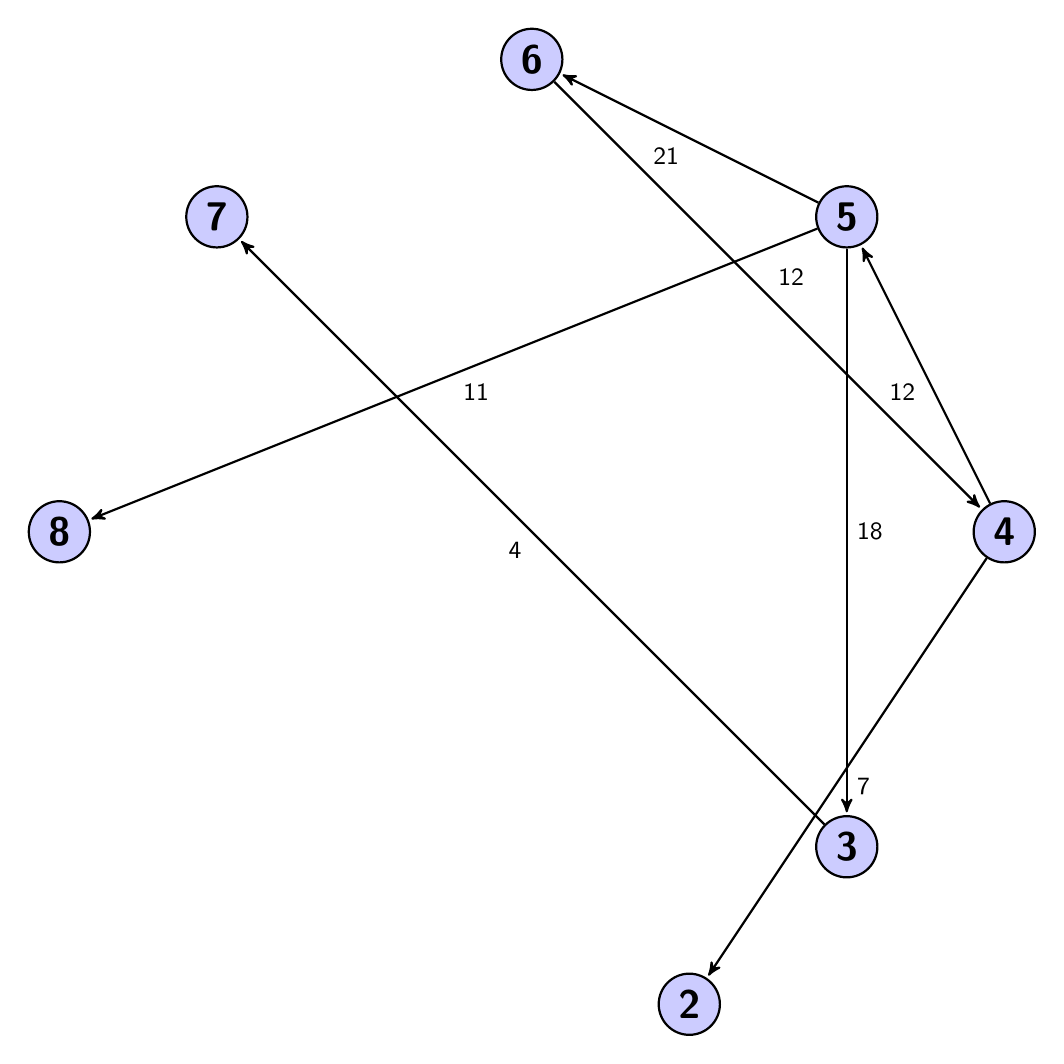
\begin{tikzpicture}[->,>=stealth',shorten >=1pt,auto,node distance=3cm,thick,main node/.style={circle,fill=blue!20,draw,font=\sffamily\Large\bfseries}]
  \node[main node] (2) at (14,0) {2};
  \node[main node] (3) at (16,2) {3};
  \node[main node] (4) at (18,6) {4};
  \node[main node] (5) at (16,10) {5};
  \node[main node] (6) at (12,12) {6};
  \node[main node] (7) at (8,10) {7};
  \node[main node] (8) at (6,6) {8};

\path[every node/.style={font=\sffamily\small}]
  (4) edge node {7} (2)
  (5) edge node {18} (3)
  (6) edge node {12} (4)
  (4) edge node {12} (5)
  (5) edge node {21} (6)
  (3) edge node {4} (7)
  (5) edge node {11} (8)
;
\end{tikzpicture}

\clearpage
path:5 6 4 2 
\\
capacity:7

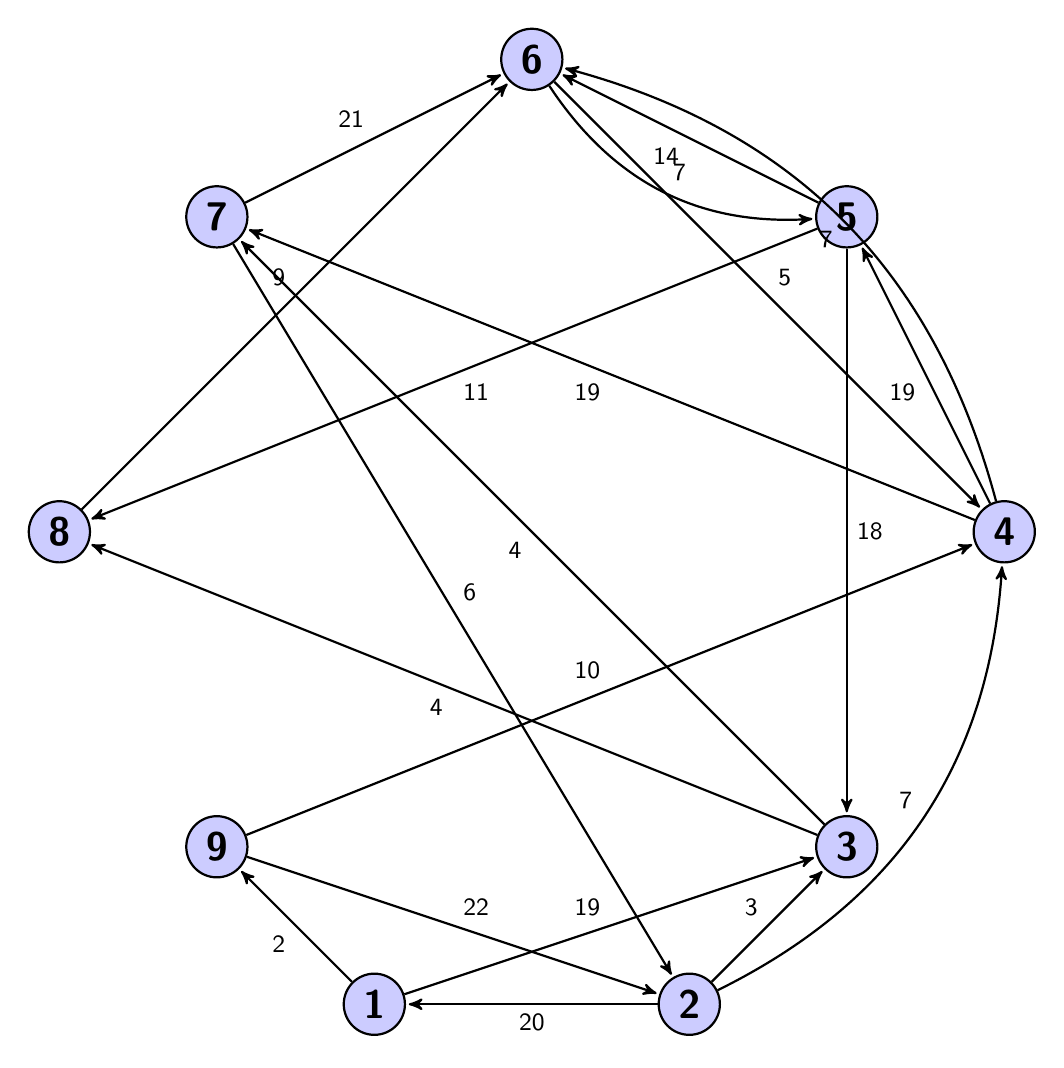
\begin{tikzpicture}[->,>=stealth',shorten >=1pt,auto,node distance=3cm,thick,main node/.style={circle,fill=blue!20,draw,font=\sffamily\Large\bfseries}]
  \node[main node] (1) at (10,0) {1};
  \node[main node] (2) at (14,0) {2};
  \node[main node] (3) at (16,2) {3};
  \node[main node] (4) at (18,6) {4};
  \node[main node] (5) at (16,10) {5};
  \node[main node] (6) at (12,12) {6};
  \node[main node] (7) at (8,10) {7};
  \node[main node] (8) at (6,6) {8};
  \node[main node] (9) at (8,2) {9};

\path[every node/.style={font=\sffamily\small}]
  (1) edge node {19} (3)
  (1) edge node {2} (9)
  (2) edge node {20} (1)
  (2) edge node {3} (3)
  (3) edge node {4} (7)
  (3) edge node {4} (8)
  (4) edge node {19} (5)
  (4) edge node {19} (7)
  (5) edge node {18} (3)
  (5) edge node {14} (6)
  (5) edge node {11} (8)
  (6) edge node {5} (4)
  (7) edge node {6} (2)
  (7) edge node {21} (6)
  (8) edge node {9} (6)
  (9) edge node {22} (2)
  (9) edge node {10} (4)
  (6) edge [bend right] node  {7} (5)
  (2) edge [bend right] node  {7} (4)
  (4) edge [bend right] node  {7} (6)
;
\end{tikzpicture}


\clearpage

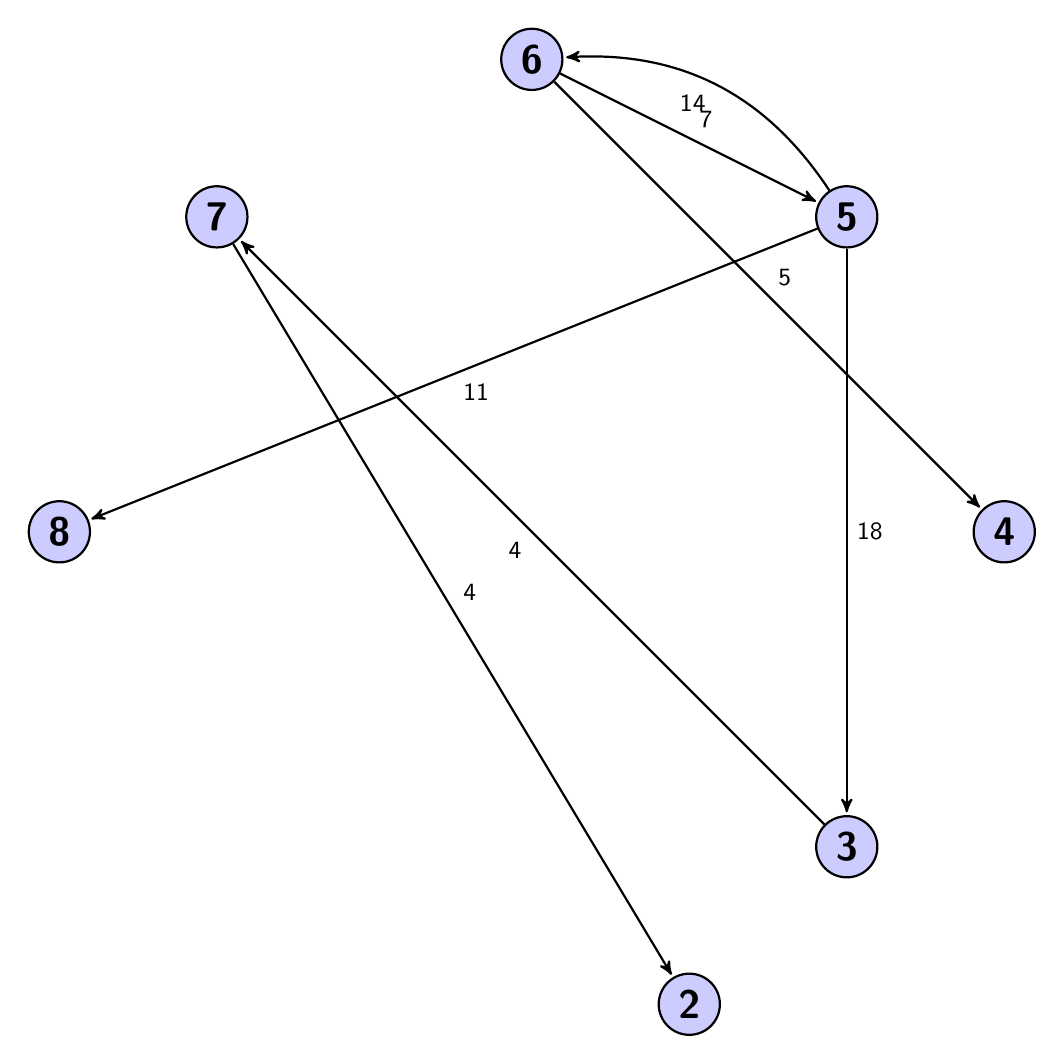
\begin{tikzpicture}[->,>=stealth',shorten >=1pt,auto,node distance=3cm,thick,main node/.style={circle,fill=blue!20,draw,font=\sffamily\Large\bfseries}]
  \node[main node] (2) at (14,0) {2};
  \node[main node] (3) at (16,2) {3};
  \node[main node] (4) at (18,6) {4};
  \node[main node] (5) at (16,10) {5};
  \node[main node] (6) at (12,12) {6};
  \node[main node] (7) at (8,10) {7};
  \node[main node] (8) at (6,6) {8};

\path[every node/.style={font=\sffamily\small}]
  (7) edge node {4} (2)
  (5) edge node {18} (3)
  (6) edge node {5} (4)
  (6) edge node {7} (5)
  (5) edge [bend right] node  {14} (6)
  (3) edge node {4} (7)
  (5) edge node {11} (8)
;
\end{tikzpicture}

\clearpage
path:5 3 7 2 
\\
capacity:4

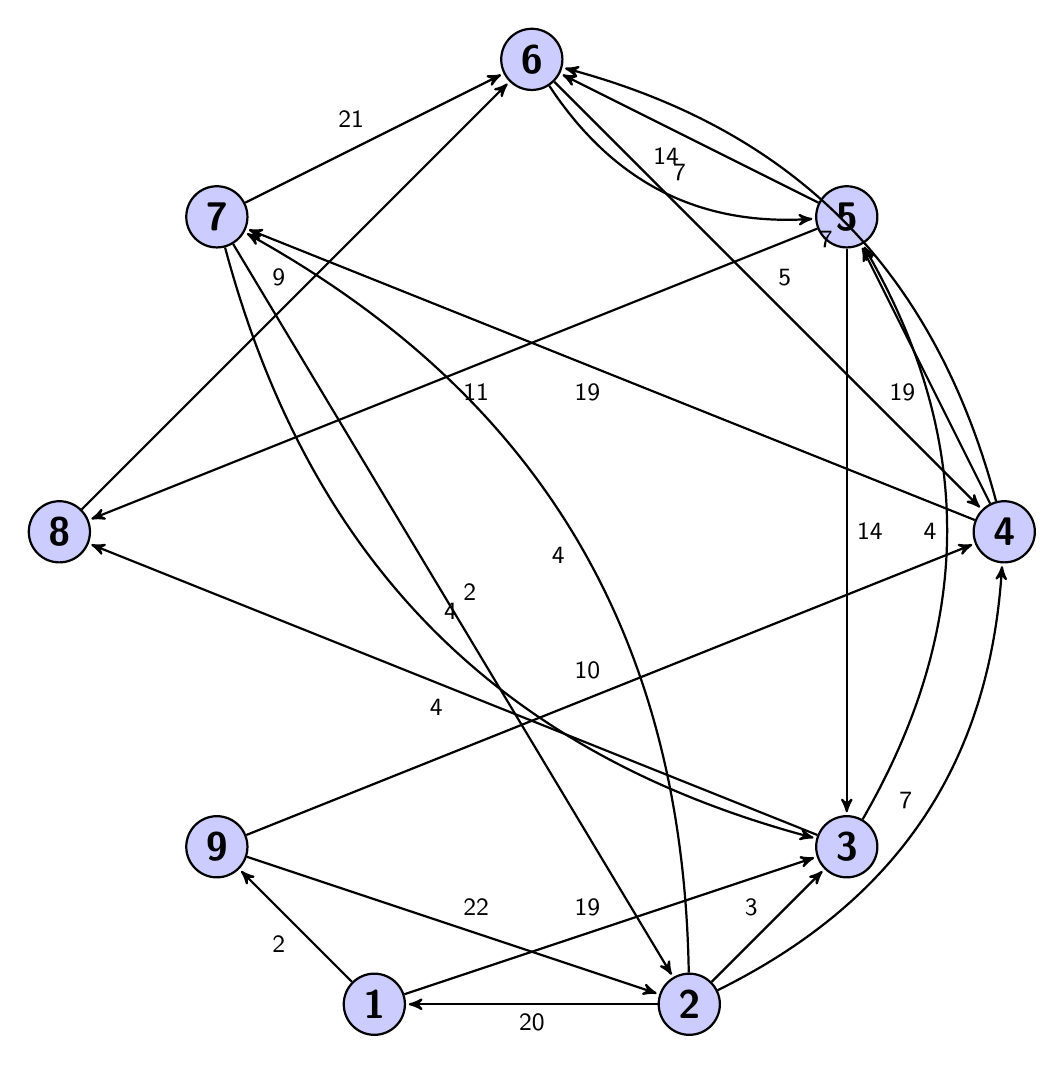
\begin{tikzpicture}[->,>=stealth',shorten >=1pt,auto,node distance=3cm,thick,main node/.style={circle,fill=blue!20,draw,font=\sffamily\Large\bfseries}]
  \node[main node] (1) at (10,0) {1};
  \node[main node] (2) at (14,0) {2};
  \node[main node] (3) at (16,2) {3};
  \node[main node] (4) at (18,6) {4};
  \node[main node] (5) at (16,10) {5};
  \node[main node] (6) at (12,12) {6};
  \node[main node] (7) at (8,10) {7};
  \node[main node] (8) at (6,6) {8};
  \node[main node] (9) at (8,2) {9};

\path[every node/.style={font=\sffamily\small}]
  (1) edge node {19} (3)
  (1) edge node {2} (9)
  (2) edge node {20} (1)
  (2) edge node {3} (3)
  (3) edge node {4} (8)
  (4) edge node {19} (5)
  (4) edge node {19} (7)
  (5) edge node {14} (3)
  (5) edge node {14} (6)
  (5) edge node {11} (8)
  (6) edge node {5} (4)
  (7) edge node {2} (2)
  (7) edge node {21} (6)
  (8) edge node {9} (6)
  (9) edge node {22} (2)
  (9) edge node {10} (4)
  (6) edge [bend right] node  {7} (5)
  (2) edge [bend right] node  {4} (7)
  (2) edge [bend right] node  {7} (4)
  (3) edge [bend right] node  {4} (5)
  (4) edge [bend right] node  {7} (6)
  (7) edge [bend right] node  {4} (3)
;
\end{tikzpicture}


\clearpage

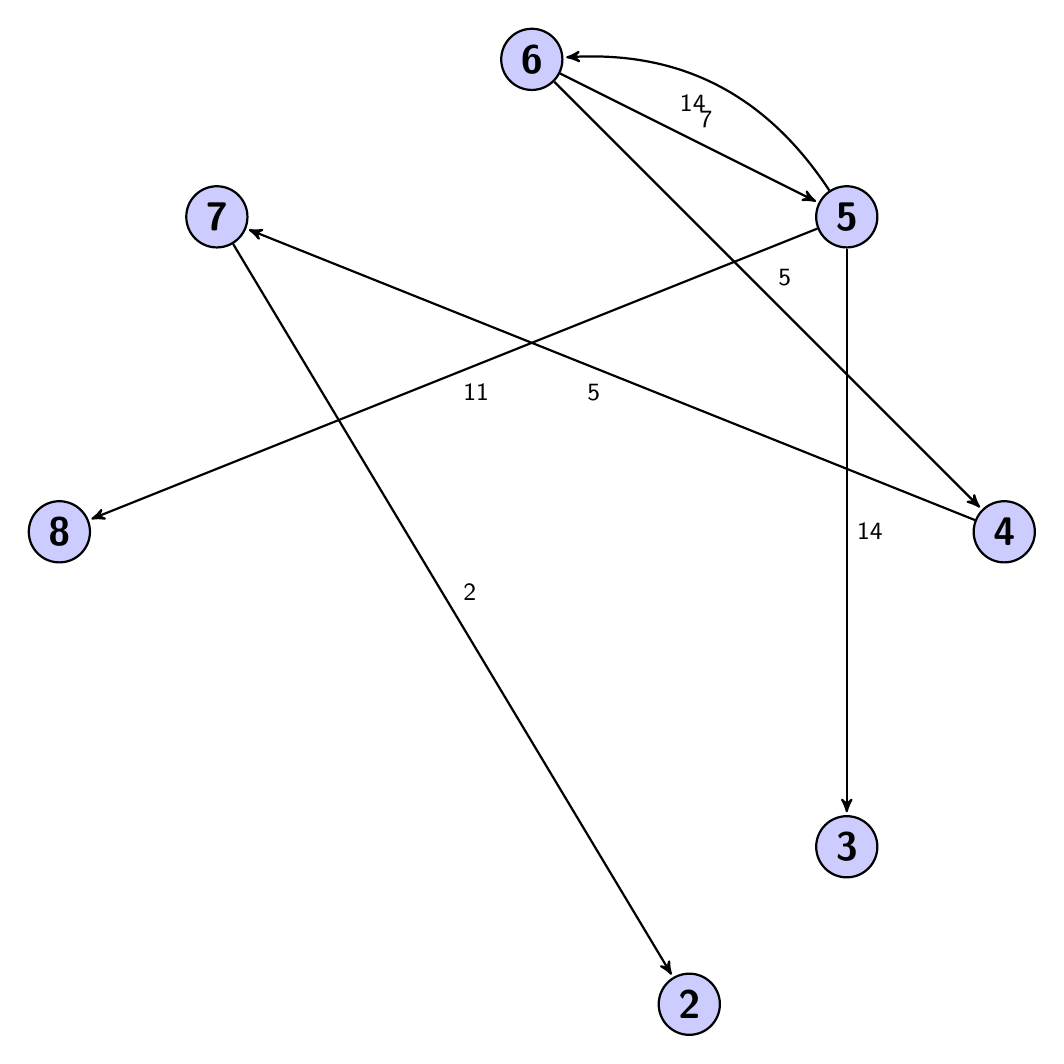
\begin{tikzpicture}[->,>=stealth',shorten >=1pt,auto,node distance=3cm,thick,main node/.style={circle,fill=blue!20,draw,font=\sffamily\Large\bfseries}]
  \node[main node] (2) at (14,0) {2};
  \node[main node] (3) at (16,2) {3};
  \node[main node] (4) at (18,6) {4};
  \node[main node] (5) at (16,10) {5};
  \node[main node] (6) at (12,12) {6};
  \node[main node] (7) at (8,10) {7};
  \node[main node] (8) at (6,6) {8};

\path[every node/.style={font=\sffamily\small}]
  (7) edge node {2} (2)
  (5) edge node {14} (3)
  (6) edge node {5} (4)
  (6) edge node {7} (5)
  (5) edge [bend right] node  {14} (6)
  (4) edge node {5} (7)
  (5) edge node {11} (8)
;
\end{tikzpicture}

\clearpage
path:5 6 4 7 2 
\\
capacity:2

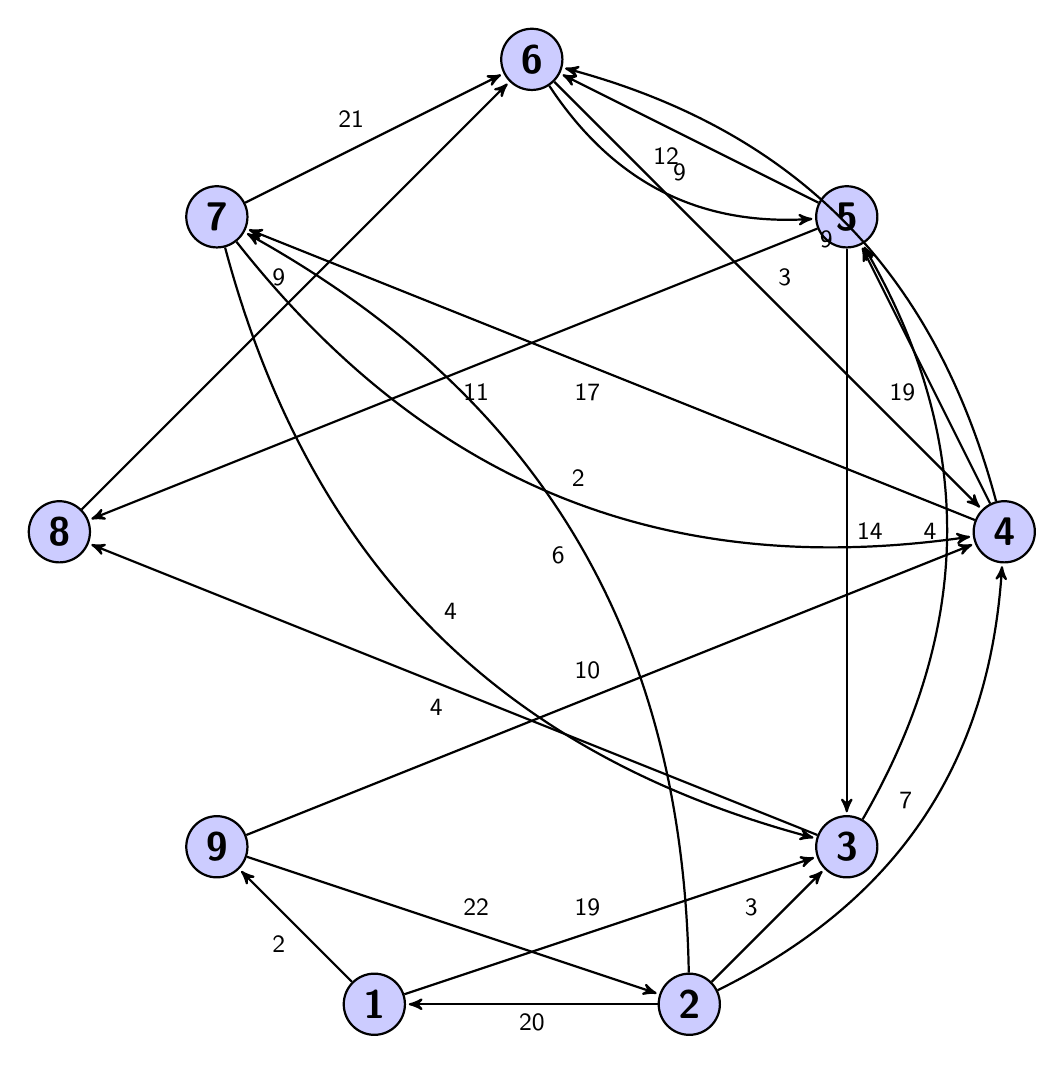
\begin{tikzpicture}[->,>=stealth',shorten >=1pt,auto,node distance=3cm,thick,main node/.style={circle,fill=blue!20,draw,font=\sffamily\Large\bfseries}]
  \node[main node] (1) at (10,0) {1};
  \node[main node] (2) at (14,0) {2};
  \node[main node] (3) at (16,2) {3};
  \node[main node] (4) at (18,6) {4};
  \node[main node] (5) at (16,10) {5};
  \node[main node] (6) at (12,12) {6};
  \node[main node] (7) at (8,10) {7};
  \node[main node] (8) at (6,6) {8};
  \node[main node] (9) at (8,2) {9};

\path[every node/.style={font=\sffamily\small}]
  (1) edge node {19} (3)
  (1) edge node {2} (9)
  (2) edge node {20} (1)
  (2) edge node {3} (3)
  (3) edge node {4} (8)
  (4) edge node {19} (5)
  (4) edge node {17} (7)
  (5) edge node {14} (3)
  (5) edge node {12} (6)
  (5) edge node {11} (8)
  (6) edge node {3} (4)
  (7) edge node {21} (6)
  (8) edge node {9} (6)
  (9) edge node {22} (2)
  (9) edge node {10} (4)
  (7) edge [bend right] node  {2} (4)
  (6) edge [bend right] node  {9} (5)
  (2) edge [bend right] node  {6} (7)
  (2) edge [bend right] node  {7} (4)
  (3) edge [bend right] node  {4} (5)
  (4) edge [bend right] node  {9} (6)
  (7) edge [bend right] node  {4} (3)
;
\end{tikzpicture}

13


%%%%%%%%%%%%%%%%%%%%%%%%%%%%%%%%%%%%%%%%%%

\end{document}  